\documentclass{ximera}

\input{../preamble.tex}

\outcome{Recognize sequences as functions.}
\outcome{Graph sequences.}
\outcome{Know terminology for sequences.}
\outcome{Compute limits of sequences.}
\outcome{Understand growth rates of basic sequences.}
\outcome{Apply the monotone convergence theorem.}


\title[Dig-In:]{Sequences as functions}

\begin{document}
\begin{abstract}
  A function from positive integers to the real numbers is a sequence.
\end{abstract}
\maketitle

Let's summarize the preceding discussion in the following definition.
\begin{definition}
  A \dfn{sequence} $(a_n)$ is, formally speaking, a real-valued
  function with domain
  \[
  \{ n \in \Z : n \ge N \},\quad \text{for some integer $N$}
  \]
  where $\Z = \{\dots, -5,-4,-3,-2,-1,0,1,2,3,4,5,\dots,\}$ is the set
  of \dfn{integers}.\index{Z@$\Z$}
\end{definition}

Stated more humbly, a sequence assigns a real number to the integers
starting with an index $N$.

When thought of as a function, the ``outputs'' of a sequence are the
\dfn{elements} of the sequence; the ``$n$th element'' is the real
number that the sequence associates to the natural number $n$, and is
usually written $a_n$. \index{sequence!element} The $n$ in the phrase
``$n$th element'' is called an \dfn{index}\index{sequence!index}; the
plural of index is either indices or indexes, depending on who you
ask.  The first index $N$ is called the \dfn{initial index}.

\begin{question}
  What explicit formula (as a function) corresponds to the sequence
  $a_n = -n/2+3$ for $n=1,2,3,\dots$?
  \begin{prompt}
    \[
    a(x) = \answer[given]{-x/2 + 3}
    \]
  \end{prompt}
\end{question}

\begin{question}
  What explicit formula (as a function) corresponds to the sequence
  $a_n = 6\left(\frac{2}{5}\right)^{n+2}$ for $n=1,2,3,\dots$?
  \begin{prompt}
    \[
    a(x) = \answer[given]{6\left(\frac{2}{5}\right)^{x+2}}
    \]
  \end{prompt}
\end{question}

Since sequences can be conceptualized as functions, and calculus is
used to study functions, we can now apply our knowledge of calculus to
sequences!

\section{Plotting sequences}

Here we plot sequences as points. Later, we will see another
interpretation.

\subsection{Plots of arithmetic sequences}

Recall that arithmetic sequences are those where the difference
between neighboring elements is constant.  Arithmetic sequences are
analogues of lines.  Consider a basic example:
\begin{image}
  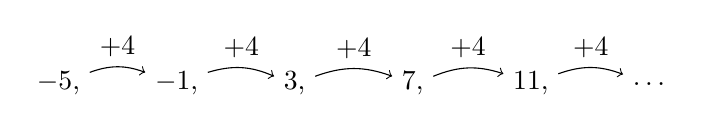
\begin{tikzpicture}[node distance=1.5cm]
    \node (a1) {$-5$,};
    \node (a2) [right of=a1] {$-1$,};
    \node (a3) [right of=a2] {$3$,};
    \node (a4) [right of=a3] {$7$,};
    \node (a5) [right of=a4] {$11$,};
    \node (a6) [right of=a5] {$\ldots$};
    
    \path[->] (a1) edge [bend left=20] node[above]{$+4$} (a2);
    \path[->] (a2) edge [bend left=20] node[above]{$+4$} (a3);
    \path[->] (a3) edge [bend left=20] node[above]{$+4$} (a4);
    \path[->] (a4) edge [bend left=20] node[above]{$+4$} (a5);
    \path[->] (a5) edge [bend left=20] node[above]{$+4$} (a6);
  \end{tikzpicture}
\end{image}

Check out a graph of the sequence:

\begin{image}
\begin{tikzpicture}
	\begin{axis}[
            domain=0:6,xmin=0,xmax=6,ymin=-9,ymax=15,
            width=4in,
            height=2in,
            axis lines =middle, xlabel=$n$, ylabel=$a$,
            xtick={1,2,...,5},
            ytick={-5,-1,...,11},
            yticklabels={$a_1 = -5$,$a_2=-1$,$a_3=3$,$a_4=7$,$a_5=11$},
            every axis y label/.style={at=(current axis.above origin),anchor=south},
            every axis x label/.style={at=(current axis.right of origin),anchor=west},
            clip=false,
            %axis on top,
          ]
          \addplot[color=penColor,fill=penColor,only marks,mark=*] coordinates{(1,-5)};  %% closed hole          
          \addplot[color=penColor,fill=penColor,only marks,mark=*] coordinates{(2,-1)};  %% closed hole          
          \addplot[color=penColor,fill=penColor,only marks,mark=*] coordinates{(3,3)};  %% closed hole          
          \addplot[color=penColor,fill=penColor,only marks,mark=*] coordinates{(4,7)};  %% closed hole          
          \addplot[color=penColor,fill=penColor,only marks,mark=*] coordinates{(5,11)};  %% closed hole  
        \end{axis}
\end{tikzpicture}
\end{image}

Here is an arithmetic sequence that decreases as its index increases.

\begin{image}
  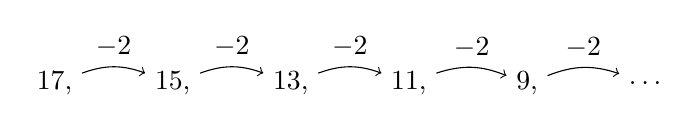
\begin{tikzpicture}[node distance=1.5cm]
    \node (a1) {$17$,};
    \node (a2) [right of=a1] {$15$,};
    \node (a3) [right of=a2] {$13$,};
    \node (a4) [right of=a3] {$11$,};
    \node (a5) [right of=a4] {$9$,};
    \node (a6) [right of=a5] {$\ldots$};

    \path[->] (a1) edge [bend left=20] node[above]{$-2$} (a2);
    \path[->] (a2) edge [bend left=20] node[above]{$-2$} (a3);
    \path[->] (a3) edge [bend left=20] node[above]{$-2$} (a4);
    \path[->] (a4) edge [bend left=20] node[above]{$-2$} (a5);
    \path[->] (a5) edge [bend left=20] node[above]{$-2$} (a6);
  \end{tikzpicture}
\end{image}

Here we see a graph:

\begin{image}
\begin{tikzpicture}
	\begin{axis}[
            domain=0:6,xmin=0,xmax=6,ymin=7,ymax=19,
            width=4in,
            height=2in,
            xtick={1,2,...,5},
            ytick={17,15,...,9},
            yticklabels={$a_1 = 17$,$a_2=15$,$a_3=13$,$a_4=11$,$a_5=9$},
            axis lines =middle, xlabel=$n$, ylabel=$a$,
            every axis y label/.style={at=(current axis.above origin),anchor=south},
            every axis x label/.style={at=(current axis.right of origin),anchor=west},
            clip=false,
            %axis on top,
          ]
          \addplot[color=penColor,fill=penColor,only marks,mark=*] coordinates{(1,17)};  %% closed hole          
          \addplot[color=penColor,fill=penColor,only marks,mark=*] coordinates{(2,15)};  %% closed hole          
          \addplot[color=penColor,fill=penColor,only marks,mark=*] coordinates{(3,13)};  %% closed hole          
          \addplot[color=penColor,fill=penColor,only marks,mark=*] coordinates{(4,11)};  %% closed hole          
          \addplot[color=penColor,fill=penColor,only marks,mark=*] coordinates{(5,9)};  %% closed hole  
        \end{axis}
\end{tikzpicture}
\end{image}


\begin{question}
  What type of curve do arithmetic sequences correspond to?
  \begin{multipleChoice}
    \choice[correct]{lines}
    \choice{parabolas}
    \choice{polynomials}
    \choice{exponential curves}
    \choice{impossible to say}
  \end{multipleChoice}
  \begin{feedback}
    Since the average growth rate of a line is constant, regardless of
    the size of the interval chosen, arithmetic sequences correspond to
    lines.
  \end{feedback}
\end{question}


\subsection{Plots of geometric sequences}

Recall that geometric sequences are those where the ratio between
neighboring elements is constant.  When this ratio is positive, a
geometric sequence corresponds to an exponential function. Consider a
basic example:
\begin{image}
    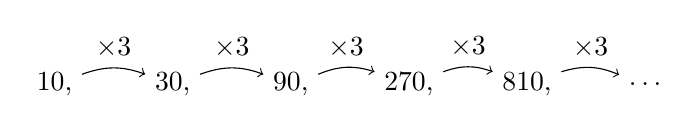
\begin{tikzpicture}[node distance=1.5cm]
    \node (a1) {$10$,};
    \node (a2) [right of=a1] {$30$,};
    \node (a3) [right of=a2] {$90$,};
    \node (a4) [right of=a3] {$270$,};
    \node (a5) [right of=a4] {$810$,};
    \node (a6) [right of=a5] {$\ldots$};

    \path[->] (a1) edge [bend left=20] node[above] {$\times 3$} (a2);
    \path[->] (a2) edge [bend left=20] node[above] {$\times 3$} (a3);
    \path[->] (a3) edge [bend left=20] node[above] {$\times 3$} (a4);
    \path[->] (a4) edge [bend left=20] node[above] {$\times 3$} (a5);
    \path[->] (a5) edge [bend left=20] node[above] {$\times 3$} (a6);
  \end{tikzpicture}
\end{image}
Let's see a graph: 
\begin{image}
\begin{tikzpicture}
	\begin{axis}[
            domain=0:6,xmin=0,xmax=6,ymin=-100,ymax=900,
            width=4in,
            height=2in,
            xtick={1,2,...,5},
            ytick={10,30,90,270,810},
            yticklabels={},%$a_1 = 10$,$a_2=30$,$a_3=90$,$a_4=270$,$a_5=810$},
            axis lines =middle, xlabel=$n$, ylabel=$a$,
            every axis y label/.style={at=(current axis.above origin),anchor=south},
            every axis x label/.style={at=(current axis.right of origin),anchor=west},
            clip=false,
            %axis on top,
          ]
          \addplot[color=penColor,fill=penColor,only marks,mark=*] coordinates{(1,10)};  %% closed hole          
          \addplot[color=penColor,fill=penColor,only marks,mark=*] coordinates{(2,30)};  %% closed hole          
          \addplot[color=penColor,fill=penColor,only marks,mark=*] coordinates{(3,90)};  %% closed hole          
          \addplot[color=penColor,fill=penColor,only marks,mark=*] coordinates{(4,270)};  %% closed hole          
          \addplot[color=penColor,fill=penColor,only marks,mark=*] coordinates{(5,810)};  %% closed hole  
        \end{axis}
\end{tikzpicture}
\end{image}

If the common ratio of a geometric sequence is between $0$ and $1$, a
geometric sequence will decrease as it progresses.

\begin{image}
  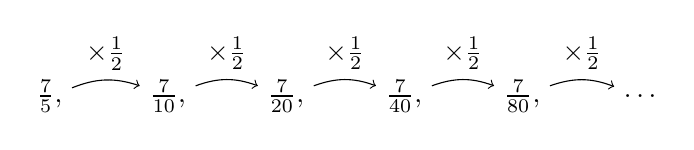
\begin{tikzpicture}[node distance=1.5cm]
    \node (a1) {$\frac{7}{5}$,};
    \node (a2) [right of=a1] {$\frac{7}{10}$,};
    \node (a3) [right of=a2] {$\frac{7}{20}$,};
    \node (a4) [right of=a3] {$\frac{7}{40}$,};
    \node (a5) [right of=a4] {$\frac{7}{80}$,};
    \node (a6) [right of=a5] {$\ldots$};
    
    \path[->] (a1) edge [bend left=20] node[above] {$\times\frac{1}{2}$} (a2);
    \path[->] (a2) edge [bend left=20] node[above] {$\times\frac{1}{2}$} (a3);
    \path[->] (a3) edge [bend left=20] node[above] {$\times\frac{1}{2}$} (a4);
    \path[->] (a4) edge [bend left=20] node[above] {$\times\frac{1}{2}$} (a5);
    \path[->] (a5) edge [bend left=20] node[above] {$\times\frac{1}{2}$} (a6);
  \end{tikzpicture}
\end{image}
Let's see a graph:
\begin{image}
\begin{tikzpicture}
	\begin{axis}[
            domain=0:6,xmin=0,xmax=6,ymin=0,ymax=2,
            width=4in,
            height=2in,
            xtick={1,2,...,5},
            ytick={1.4,.7,.35,.175,.0875},
            yticklabels={},%$a_1 = 10$,$a_2=30$,$a_3=90$,$a_4=270$,$a_5=810$},
            axis lines =middle, xlabel=$n$, ylabel=$a$,
            every axis y label/.style={at=(current axis.above origin),anchor=south},
            every axis x label/.style={at=(current axis.right of origin),anchor=west},
            clip=false,
            %axis on top,
          ]
          \addplot[color=penColor,fill=penColor,only marks,mark=*] coordinates{(1,7/5)};  %% closed hole          
          \addplot[color=penColor,fill=penColor,only marks,mark=*] coordinates{(2,7/10)};  %% closed hole          
          \addplot[color=penColor,fill=penColor,only marks,mark=*] coordinates{(3,7/20)};  %% closed hole          
          \addplot[color=penColor,fill=penColor,only marks,mark=*] coordinates{(4,7/40)};  %% closed hole          
          \addplot[color=penColor,fill=penColor,only marks,mark=*] coordinates{(5,7/80)};  %% closed hole  
        \end{axis}
\end{tikzpicture}
\end{image}


\begin{question}
  When the common ratio between successive elements is positive, what
  type of curves do geometric sequence correspond to?
  \begin{multipleChoice}
    \choice{lines}
    \choice{parabolas}
    \choice{polynomials}
    \choice[correct]{exponential curves}
    \choice{impossible to say}
  \end{multipleChoice}
  \begin{feedback}
  If a geometric sequence is expressed as $a_n = a_1 \cdot r^{n-1}$,
  then in function notation we have $a(x) = a_1 \cdot r^{x-1}$, an
  exponential function.
  \end{feedback}
\end{question}



On the other hand, if the common ration between sucessive elements of
a geometric sequence is \textbf{not} positive, then something
interesting happens. Check out this example:
\begin{image}
  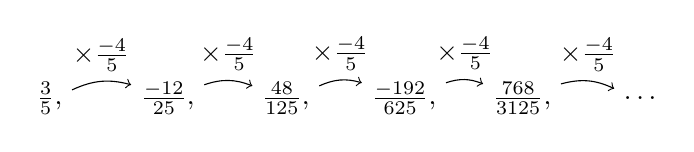
\begin{tikzpicture}[node distance=1.5cm]
    \node (a1) {$\frac{3}{5}$,};
    \node (a2) [right of=a1] {$\frac{-12}{25}$,};
    \node (a3) [right of=a2] {$\frac{48}{125}$,};
    \node (a4) [right of=a3] {$\frac{-192}{625}$,};L
    \node (a5) [right of=a4] {$\frac{768}{3125}$,};
    \node (a6) [right of=a5] {$\ldots$};
    
    \path[->] (a1) edge [bend left=20] node[above] {$\times\frac{-4}{5}$} (a2);
    \path[->] (a2) edge [bend left=20] node[above] {$\times\frac{-4}{5}$} (a3);
    \path[->] (a3) edge [bend left=20] node[above] {$\times\frac{-4}{5}$} (a4);
    \path[->] (a4) edge [bend left=20] node[above] {$\times\frac{-4}{5}$} (a5);
    \path[->] (a5) edge [bend left=20] node[above] {$\times\frac{-4}{5}$} (a6);
  \end{tikzpicture}
\end{image}
Let's see a graph:
\begin{image}
\begin{tikzpicture}
	\begin{axis}[
            domain=0:6,xmin=0,xmax=6,ymin=-.7,ymax=.7,
            width=4in,
            height=2in,
            xtick={1,2,...,5},
            ytick={.6,-.48,.384,-.3072,.24576},
            yticklabels={},%$a_1 = 10$,$a_2=30$,$a_3=90$,$a_4=270$,$a_5=810$},
            axis lines =middle, xlabel=$n$, ylabel=$a$,
            every axis y label/.style={at=(current axis.above origin),anchor=south},
            every axis x label/.style={at=(current axis.right of origin),anchor=west},
            clip=false,
            %axis on top,
          ]
          \addplot[color=penColor,fill=penColor,only marks,mark=*] coordinates{(1,3/5)};  %% closed hole          
          \addplot[color=penColor,fill=penColor,only marks,mark=*] coordinates{(2,-12/25)};  %% closed hole          
          \addplot[color=penColor,fill=penColor,only marks,mark=*] coordinates{(3,48/125)};  %% closed hole          
          \addplot[color=penColor,fill=penColor,only marks,mark=*] coordinates{(4,-192/625)};  %% closed hole          
          \addplot[color=penColor,fill=penColor,only marks,mark=*] coordinates{(5,768/3125)};  %% closed hole  
        \end{axis}
\end{tikzpicture}
\end{image}
The sign of this sequence alternates! 

\subsection{Monotonicity}

We'd like some terminology with which to describe features we might
notice about sequences.  Here is some of that terminology.

\begin{definition}
  A sequence is called \dfn{increasing}\index{sequence!increasing} if
  $ a_n<a_{n+1}$ for all $n$.  It is called
  \dfn{nondecreasing}\index{sequence!nondecreasing} if $ a_n\le
  a_{n+1}$ for all $n$.

  Similarly a sequence is \dfn{decreasing}\index{sequence!decreasing}
  if $ a_n>a_{n+1}$ for all $n$ and
  \dfn{nonincreasing}\index{sequence!nonincreasing} if $ a_n\ge
  a_{n+1}$ for all $n$.
\end{definition}

Lots of facts are true for sequences which are either increasing or
decreasing; to talk about this situation without constantly saying
``either increasing or decreasing,'' we can make up a single word to
cover both cases.
\begin{definition}
  If a sequence is
  \begin{itemize}
  \item increasing, or
  \item nondecreasing, or
  \item decreasing, or
  \item nonincreasing,
  \end{itemize}
  it is said to be \dfn{monotonic}\index{sequence!monotonic}.
\end{definition}


Let's see some examples of sequences which are monotonic.
\begin{example}
The sequence $ a_n = {2^n-1\over2^n}$ which starts
\[
  \frac{1}{2},\quad \frac{3}{4},\quad \frac{7}{8},\quad \frac{15}{16},\quad \ldots,
\]
is increasing.  On the other hand, the sequence $ b_n = \frac{n+1}{n}$, which starts
\[ 
  \frac{2}{1},\quad\frac{3}{2},\quad\frac{4}{3},\quad\frac{5}{4},\quad\ldots,
\]
is decreasing.
\end{example}

BADBAD QUESTION MONOTONIC ANALYTIC


Sometimes we can say that the sequence doesn't get too big or too
small, in this case we say the sequence is \textit{bounded}

\begin{definition}
  \label{definition:sequence-bounded}
  A sequence $(a_n)$ is \dfn{bounded above}\index{sequence!bounded
    above} if there is some number $M$ so that for all $n$, we have $
  a_n\le M$.  Likewise, a sequence $(a_n)$ is \dfn{bounded
    below}\index{sequence!bounded below} if there is some number $M$
  so that for every $n$, we have $ a_n\ge M$.

If a sequence is both bounded above and bounded below, the sequence is said
to be \dfn{bounded}\index{sequence!bounded}.
\end{definition}





\begin{question}
  To say that the sequence $a_n$ is ``bounded below'' is to say what?

    \begin{hint}
      The definition begins by asserting the existence of some bound $M$.
    \end{hint}
    \begin{hint}
      The bound is a real number, meaning $M \in \mathbb{R}$.
    \end{hint}
    \begin{hint}
      So the definition begins ``there exists an $M \in \mathbb{R}$\ldots''
    \end{hint}
    \begin{hint}
      The bound must hold for all terms in the sequence.
    \end{hint}
    \begin{hint}
      So we will assert something for all indexes $n \in \mathbb{N}$.
    \end{hint}
    \begin{hint}
      The definition begins ``there exists an $M \in \mathbb{R}$, so that for all $n \in \mathbb{N}$, \ldots''
    \end{hint}
    \begin{hint}
      For a particular term $a_n$ to be bounded below by $M$ just means that $a_n \ge M$.
    \end{hint}
    \begin{hint}
      Altogether then, being bounded below means ``there exists an $M \in \mathbb{R}$, so that for all $n \in \mathbb{N}$, we have $a_n \ge M$.''  Sometimes you might see this ending with $ a_n > M $, but that is a difference which does not affect which sequences are bounded below.
      
    \end{hint}
    
    \begin{multipleChoice}
      \choice[correct]{There exists an $M \in \mathbb{R}$, so that for all $n \in \mathbb{N}$, we have $a_n \ge M$.}
      \choice{There exists an $n \in \mathbb{N}$, so that for all $M \in \mathbb{R}$, we have $a_n \ge M$.}
      \choice{For all $M \in \mathbb{R}$, there exists an $n \in \mathbb{N}$, so that $a_n \ge M$.}
      \choice{For all $n \in \mathbb{N}$, there exists an $M \in \mathbb{R}$, so that $a_n \ge M$.}
      \choice{There exists an $M \in \mathbb{R}$, so that for all $n \in \mathbb{N}$, we have $a_n \le M$.}
    \end{multipleChoice}

\end{question}
            
If a sequence $
\{a_n\}_{n=0}^\infty$ is increasing or non-decreasing it is bounded
below (by $ a_0$), and if it is decreasing or non-increasing it is
bounded above (by $ a_0$).

\begin{question}
  Consider the sequence $b_{n} = -n^{2} + 5 \, n - 5$.  Is the sequence bounded above?  Bounded below?

    \begin{hint}
      Consider the coefficient on $n^{2}$ in $b_{n} = -n^{2} + 5 \, n - 5$, which is $-1$.
    \end{hint}
    \begin{hint}
      Since the leading term's coefficient is negative, when $n$ is large, $b_{n}$ is very negative.
    \end{hint}
    \begin{hint}
      Consequently, the sequence is not bounded below.
    \end{hint}
    \begin{hint}
      At least for $n$ large, the sequence is decreasing.
    \end{hint}
    \begin{hint}
      Consequently, the sequence is bounded above.
    \end{hint}
    \begin{hint}
      Altogether then, the sequence is bounded above, but not below.
    \end{hint}

    \begin{multipleChoice}
      \choice[correct]{Bounded above, but not bounded below.}
      \choice{Bounded below, but not bounded above.}
      \choice{Bounded above and bounded below.}
      \choice{Bounded neither above nor below.}
    \end{multipleChoice}

\end{question}





\section{Limits of sequences}

Since sequences are essentially \dfn{discrete}, meaning that the points
are separate and distinct, the notion of a ``limit at a point'' cannot
be made to really make sense. However, limits at \textit{infinity} are
a different story.


We've seen a lot of sequences, and already there are a few things we
might notice.  For instance, the arithmetic progression
\[
1,\quad 8,\quad 15,\quad 22,\quad 29,\quad 36,\quad 43,\quad 50,\quad 57,\quad 64,\quad 71,\quad 78,\quad 85,\quad 92,\quad \ldots
\]
just keeps getting bigger and bigger.  No matter how large a number
you think of, if I add enough $7$'s to $1$, eventually I will surpass
the giant number you thought of.  On the other hand, the elements in a
geometric progression where each element is half the previous element,
namely
\[
\frac{1}{2},\quad \frac{1}{4},\quad \frac{1}{8},\quad \frac{1}{16},\quad \frac{1}{32},\quad \frac{1}{64},\quad \frac{1}{128},\quad \frac{1}{256},\quad \frac{1}{512},\quad \frac{1}{1024},\quad \ldots ,
\]
are getting closer and closer to zero.  No matter how close you stand
near but not at zero, eventually this geometric sequence gets even
closer than you are to zero.

%\youtube{https://www.youtube.com/watch?v=PRTjvMA2nCY}

These two sequences have very different stories.  One shoots off to
infinity; the other zooms in towards zero.  Mathematics is not just
about numbers; mathematics provides tools for talking about the
qualitative features of the numbers we deal with.  What about the two
sequences we just considered?  They are qualitatively very different.
The first ``goes to'' infinity; the second ``goes to'' zero.

In short, given a sequence, it is helpful to be able to say something
qualitative about it; we may want to address the question such as
``what happens after a while?'' Formally, when faced with a sequence,
we are interested in the limit
\[
\lim_{i\to \infty} f(i) = \lim_{i\to\infty} a_i.
\]
Earlier you've studied a similar question about
\[
\lim_{x\to\infty} f(x)
\]
when $x$ is a variable taking on real values; now, we simply want to
restrict the ``input'' values to be integers. No significant
difference is required in the definition of limit, except that we
specify, perhaps implicitly, that the variable is an integer.

\begin{definition}\index{limit of a sequence}
\label{definition:limit-of-a-sequence}
Suppose that $\left(a_n\right)$ is a sequence.
To say that $\lim_{n\to \infty}a_n=L$ is to say that \\
\null\quad for every $\epsilon>0$, \\
\null\quad\quad there is an $N > 0$, \\
\null\quad so that whenever $n>N$, \\
\null\quad\quad we have $|a_n-L|<\epsilon$. \\
If $\lim_{n\to\infty}a_n=L$ we say that the sequence
\dfn{converges}\index{convergent
  sequence}\index{sequence!convergent}.  If there is no finite value $L$ so
that $\lim_{n\to\infty}a_n = L$, then we say that the limit
\dfn{does not exist}, or equivalently that the sequence
\dfn{diverges}\index{divergent sequence}\index{sequence!divergent}.
\end{definition} 

\begin{question}
  To say that the sequence $a_n$ converges to $L$ means what?  In other words, what is the definition of the statement $\lim_{n \to \infty} a_n = L$?

    \begin{hint}
      We are trying to make precise the idea that, eventually, all the elements of the sequence $a_n$ are as close as we want to $L$.
    \end{hint}
    \begin{hint}
      To measure closeness to $L$, we will use a positive real number $\epsilon$.
    \end{hint}
    \begin{hint}
      We must achieve any desired degree of closeness, so we will make a statement which is true for any positive real number $\epsilon$.
    \end{hint}
    \begin{hint}
      In other words, the definition will begin ``For every positive real number $\epsilon > 0$\ldots''
    \end{hint}
    \begin{hint}
      We now must make precise the idea of ``eventually'' close.
    \end{hint}
    \begin{hint}
      We use a whole number $N$ to capture the idea of ``sufficiently large'' values of $n$.
    \end{hint}
    \begin{hint}
      Specifically, the definition will begin ``For every positive real number $\epsilon > 0$, there exists an $N \in \mathbb{N}$\ldots''
    \end{hint}
    \begin{hint}
      The ``sufficiently large'' value of $n$ is any value which is at least as large as $N$.
    \end{hint}
    \begin{hint}
      So we will only consider those $n$ for which $n \ge N$.
    \end{hint}
    \begin{hint}
      Thus the definition goes ``For every positive real number $\epsilon > 0$, there exists an $N \in \mathbb{N}$ so that whenever $n \ge N$\ldots''
    \end{hint}
    \begin{hint}
      What happens ``eventually'' is that elements of the sequence are close to $L$.  How close?  Within $\epsilon$.
    \end{hint}
    \begin{hint}
      The quantity $|a_n - L|$ is the distance between $a_n$ and $L$.
    \end{hint}
    \begin{hint}
      To say that $a_n$ is within $\epsilon$ of $L$ is to say that $|a_n - L| < \epsilon$.
    \end{hint}
    \begin{hint}
      Therefore the definition is ``For every positive real number $\epsilon > 0$ there exists an $N \in \mathbb{N}$ so that whenever $n \ge N$, we have $ |a_n - L| < \epsilon $.''
    \end{hint}

    \begin{multipleChoice}
      \choice[correct]{For every positive real number $\epsilon > 0$ there exists an $N \in \mathbb{N}$ so that whenever $n \ge N$, we have $ |a_n - L| < \epsilon $.}
      \choice{For every real number $\epsilon > 0$ there exists an $N \in \mathbb{N}$ so that $ |a_N - L| < \epsilon $.}
      \choice{For every real number $\epsilon \in \mathbb{R}$ there exists an $N \in \mathbb{N}$ so that whenever $n \ge N$, we have $ |a_n - L| < \epsilon $.}
      \choice{For every whole number $N > 0$ there exists a positive real number $\epsilon > 0$ so that whenever $n \ge N$, we have $ |a_n - L| < \epsilon $.}
      \choice{For every whole number $N > 0$ there exists a real number $\epsilon \in \mathbb{R}$ so that whenever $n \ge N$, we have $ |a_n - L| < \epsilon $.}
    \end{multipleChoice}
              

  The definition of limit can be written as if it were poetry with
  line breaks and all.  Like the best of poems, it deserves to be
  memorized, performed, internalized.  Humanity struggled for millenia
  to find the wisdom contained in this definition.
\end{question}

\begin{warning}
  In the case that $\lim_{n \to \infty} a_n = \infty$, we say that
  $(a_n)$ diverges, or perhaps more precisely, we say $(a_n)$ diverges to
  infinity.  The only time we say that a sequence converges is when
  the limit exists and is equal to a \textit{finite} value.
\end{warning}

\youtube{https://www.youtube.com/watch?v=0UCRZAsIkXM}

One way to compute the limit of a sequence is to compute the limit of
a function.
\begin{theorem}
  \label{theorem:compute-limit-of-sequence-via-function}
  Let $f(x)$ be a real-valued function.  If $a_n = f(n)$ defines a
  sequence $(a_n)$ and if $\lim_{x\to\infty}f(x)=L$ in the sense of Calculus
  One, then $\lim_{n\to\infty} a_n=L$ as well.
\end{theorem}



\begin{question}
  Consider the sequence given by the rule \[b_{n} = \frac{ 3 \, n + 9 }{ 4 \, n + 20 }.\]  For which value of $N$ is it the case that whenever $n \ge N$ we have that $b_{n}$ is within $1/50$ of $3/4$?

    \begin{hint}
      There can only be one right answer.
    \end{hint}
    \begin{hint}
      So the answer is either $N = 69$ or ``none of these.''
    \end{hint}
    \begin{hint}
      Note that $b_{69} = \frac{27}{37}$.
    \end{hint}
    \begin{hint}
      Consequently, $\left| b_{69} -  \frac{3}{4} \right| = \frac{3}{148} \ge \frac{1}{50}$.
    \end{hint}
    \begin{hint}
      So the answer must be ``none of these.''
    \end{hint}

    \begin{multipleChoice}
      \choice[correct]{None of these choices for $N$ is large enough.}
      \choice{$N = 69 $}
      \choice{$N = 67 $}
      \choice{$N = 65 $}
      \choice{$N = 63 $}
    \end{multipleChoice}

\end{question}

But it is important to note that the converse of this theorem is not
true; \label{sidenote:raining-converse}the \dfn{converse} of a
statement is what you get when you swap the assumption and the
conclusion; the converse of ``if it is raining, then it is cloudy'' is
the statement ``if it is cloudy, then it is raining.''  Which of those
statements is true?.

To show the converse is not true, it is enough to provide a single
example where it fails.  Here's the counterexample.  Recall an
instance of (a potential) general rule being broken is called a
\dfn{counterexample}.  This is a popular element among
mathematicians and philosophers.

\begin{example}
  Consider the sequence $(a_n)$ given by the rule $a_n = f(n)=\sin(n\pi)$.  This is the sequence
$$
  \sin(0\pi),\quad \sin(1\pi),\quad\sin(2\pi),\quad\sin(3\pi),\quad\ldots,
$$
which is just the sequence $0, 0, 0, 0, \ldots$ since $\sin(n\pi)=0$
whenever $n$ is an integer.  Since the sequence is just the constant sequence, we have
$$
\lim_{n\to\infty} f(n)= \lim_{n\to\infty} 0 = 0. 
$$But $\lim_{x\to\infty}f(x)$, when $x$ is real, does not exist: as $x$ gets
bigger and bigger, the values $\sin(x\pi)$ do not get closer and
closer to a single value, but instead oscillate between $-1$ and $1$.
\end{example} 

Here's some general advice. If you want to know $\lim_{n\to\infty}
a_n$, you might first think of a function $f(x)$ where $a_n = f(n)$,
and then attempt to compute $\lim_{x\to\infty}f(x)$.  If the limit
of the function exists, then it is equal to the limit of the sequence.
But, if for some reason $\lim_{x\to\infty}f(x)$ does not exist, it
may nevertheless still be the case that $\lim_{n\to\infty}f(n)$
exists---you'll just have to figure out another way to compute it.

\section{Monotone convergence}

\begin{explanation}
which amounts to the same thing.  It is helpful trick here to think of
the ratio between subsequent terms, since the factorials end up
canceling nicely.  In particular,
\begin{align*}
  {a_{n+1}\over a_n} &= {(n+1)!\over (n+1)^{n+1}}{n^n\over n!} \\
  &= {(n+1)!\over n!}{n^n\over (n+1)^{n+1}} \\
  &= {n+1\over n+1}\left({n\over n+1}\right)^n
  &= \left({n\over n+1}\right)^n < 1.
\end{align*}
  Note that the sequence is bounded below, since every term is positive.

  Because the sequence is decreasing and bounded below, it converges.
  Indeed, an EXERCISE BADBAD asks you to compute the limit.
\end{explanation}

These sorts of arguments involving the ratio of subsequent terms will
come up again in a big way when we consider the ratio test.  Stay
tuned!

\subsection{Sample problem}

\begin{question}
  Consider the sequence $a_{n}$.  Suppose you know that for all $n >
  1$,
  \[
  -6 \le a_{n} \le 0
  \]
  and $a_{1} = 2$, and $a_{2} = -1$, and that the sequence is
  nonincreasing.  Does the sequence converge?
  \begin{hint}
    Since the sequence is nonincreasing, the sequence is monotone.
  \end{hint}
  \begin{hint}
    Since for all $n \ge 1$, we have $a_{n} \ge -6$, the sequence is
    bounded below.
  \end{hint}
  \begin{hint}
    So by the Monotone Convergence Theorem, the sequence converges to
    some value; let us call it $L$.
  \end{hint}
  \begin{hint}
    Now consider the direction in which the sequence is heading.
  \end{hint}
  \begin{hint}
    Since the sequence is nonincreasing, for all $n \ge 2$, we have
    $-6 \le a_{n} \le -1$.
  \end{hint}
  \begin{hint}
    The limit $L$ must be in that interval as well.
  \end{hint}
  \begin{hint}
    Therefore the sequence converges to a value $L$ so that $-6 \le L
    \le -1$.
  \end{hint}
  \begin{multipleChoice}
    \choice[correct]{Yes, with limit between $-6$ and $-1$.}
    \choice{No, the sequence does not converge.}
    \choice{Yes, with limit between $-1$ and $0$.}
  \end{multipleChoice}
\end{question}




\section{Derivatives}

arithmetic vs geometric.

logarithmic derivative


L'H\^opital

\section{Integrals}







\section{New from old}

Given a sequence, one way to build a new sequence is to start with the
old sequence, but then throw away a whole bunch of elements.  For
instance, if we started with the sequence of perfect squares
$$
1,\quad 4,\quad 9,\quad 16,\quad 25,\quad 36,\quad 49,\quad 64,\quad 81,\quad\ldots
$$
we could throw away all the odd-indexed elements, and be left with
$$
4,\quad 16,\quad 36,\quad 64,\quad 100,\quad 144,\quad 196,\quad 256,\quad 324,\quad 400,\quad 484,\quad\ldots
$$
We say that this latter sequence is a
\dfn{subsequence}\index{sequence!subsequence}\index{subsequence}
of the original sequence.  Here is a precise definition.

\begin{definition}
  Suppose $(a_n)$ is a sequence with initial index $N$, and suppose we have a sequence of integers $(n_i)$ so that
  $$
  N \le n_1 < n_2 < n_3 < n_4 < n_5 < \cdots 
  $$
  Then the sequence $(b_i)$ given by $b_i = a_{n_i}$ is said to be a \dfn{subsequence}\index{sequence!subsequence}\index{subsequence}
  of the sequence $a_n$.
\end{definition}

\youtube{http://www.youtube.com/watch?v=OYRRFRzf12o}

Limits are telling the story of ``what happens'' to a sequence.  If
the elements of a sequence can be made as close as desired to a limiting
value $L$, then the subsequence must share that same fate.

\begin{theorem}
  \label{theorem:subsequence-same-limit}
  If $(b_i)$ is a subsequence of the convergent sequence $(a_n)$, then
  $\lim_{i \to \infty} b_i = \lim_{n \to \infty} a_n$.
\end{theorem}

Of course, just because a subsequence converges does not mean that the
larger sequence converges, too.  We'll see this again in more detail,
but we'll discuss it briefly now.

\begin{example}
Find a convergent subsequence of the sequence $(a_n)$ given by the rule $a_n = (-1)^n$.
\end{example}

\begin{explanation}
Note that the sequence $(a_n)$ does not converge.  But by considering the sequence of indexes $n_i = 2 \cdot i$, we can build a subsequence
$$
b_i = a_{n_i} = a_{2i} = (-1)^{2i} = 1,
$$
which is a constant sequence, so it converges to 1.
\end{explanation}

There are other subsequences of $a_n = (-1)^n$ which converge but do
\textit{not} converge to one.  For instance, the subsequence of odd
indexed elements is the constant sequence $c_n = -1$, which converges to
$-1$.  For that matter, the fact that there are convergent
subsequences with distinct limits perhaps explains why the original
sequence $(a_n)$ does not converge.  Let's formalize this.

\begin{corollary}
  \label{corollary:different-subsequences-then-diverge}

  Suppose $(b_i)$ and $(c_i)$ are convergent subsequences of the sequence $(a_n)$, but
  $$
  \lim_{i \to \infty} b_i \neq \lim_{i \to \infty} c_i.
  $$
  Then the sequence $(a_n)$ does not converge.
\end{corollary}

\begin{proof}
  Suppose, on the contrary, the sequence $(a_n)$ did converge.  Then,
  since all subsequences approach the same limit, the subsequence
  $(b_i)$ would converge, too, and
  $$
  \lim_{i \to \infty} b_i = \lim_{n \to \infty} a_n.
  $$
  Again %by Theorem~\xrefn{theorem:subsequence-same-limit},
  the subsequence
  $(c_i)$ would converge, too, and
  $$
  \lim_{i \to \infty} c_i = \lim_{n \to \infty} a_n.
  $$
  But then $\lim_{i \to \infty} b_i = \lim_{i \to \infty} c_i$,
  which is exactly what we are supposing doesn't happen!  To avoid
  this contradiction, it must be that our original assumption that
  $(a_n)$ converged was incorrect; in short, the sequence $(a_n)$ does
  not converge.
\end{proof}





\end{document}
